\documentclass[a4paper,11pt]{article}

\usepackage{amsfonts}
\usepackage{amsmath}
\usepackage{amsthm}
\usepackage{amssymb}
\usepackage{graphicx}

%\usepackage{fontspec}
%\setmainfont{Times New Roman}

\usepackage[american]{babel}
\usepackage{csquotes}
\usepackage[style=apa,natbib=true,backend=biber]{biblatex}
\DeclareLanguageMapping{american}{american-apa}
\addbibresource{Polarization.bib}

\usepackage[colorlinks,allcolors=blue]{hyperref}
\hypersetup{%
    pdftitle={Is Technology Polarizing the Australian Work Force?},%
    pdfauthor={Alex Cooper},%
    pdfsubject={An analysis of one determinant of inequality in Australia.},%
    pdfkeywords={labor, polarization, routinization, SBTC, inequality},%
}
\ExecuteBibliographyOptions{doi=false}
\newbibmacro{string+doi}[1]{%
  \iffieldundef{doi}{#1}{\href{http://dx.doi.org/\thefield{doi}}{#1}}}
\DeclareFieldFormat{title}{\usebibmacro{string+doi}{\mkbibemph{#1}}}
\DeclareFieldFormat[article]{title}{\usebibmacro{string+doi}{\mkbibquote{#1}}}
\renewcommand{\bibfont}{\normalfont\small}

\renewcommand{\H}{\mathcal{H}}
\renewcommand{\L}{\mathcal{L}}

\title{Is Technology Polarizing the Australian Work Force?}
\author{Alex Cooper}
\date{August, 2013}

\begin{document}
\maketitle

This research is motivated by the observation that the income distribution for Australian workers has widened over the past 30 years. Although there are many possible explanations for this development, we focus on just one major development: the rapid rise of computer technology in the work force. We document some major trends in wage trends, and show that the standard model used to analyze the rise of technology in the work force explains some, but not all, of the trends observed in the data. In this preliminary report, we lay the ground work for an alternative model, first proposed by \citet{Levy2003}, which has been used with success in foreign labour markets. We explain how this model will be used to analyze the changing nature of the task content of the Australian work force.

The second half of the 20th century has witnessed tremendous change for Australian workers. Since 1973, average real per capita incomes have approximately doubled \citep{NA20124}, and the number of jobs has increased by over three million \citep{LFSApr2013}. During the same period, top percentile wage growth has far outstripped that of lower-wage earners \citep{Atkinson1997,Borland1999}. And although income inequality in Australia fell somewhat between the 1950's and 1970's, it has since risen consistently for the last 30 years \citep{Leigh2005,Gaston2009}.

There is a large literature studying the rise of wage inequality in Australia. Empirical studies have confirmed that both individual-level and household-level inequality have been rising since the 1980s \citep{Borland1999,Leigh2005,Gaston2009}. A number of studies exist on the task content of Australian jobs \citep{Esposto2012a}, and the change over time of the skill intensity of various professions \citep{Esposto2012, Esposto2012a}. Although ICT use and globalization have been found to Granger (non-)cause rising inequality \citep{Gaston2009}, no studies have tested whether workers' skill allocation is the channel through which this change has occurred.

Although mechanical computers and computation aids (the abacus, for instance), have been available for centuries, it was only in the post-war era, with the arrival of electronic computation, that significant gains have been made. \citet{Nordhaus2007} estimates that, between 1946 and 2006, the cost per computation decreased by a factor of {\em seven trillion,} and the cost of data storage fell at a comparable rate. The falling cost of computation opened up new avenues for research in information technology, so that even as computation became cheaper, new and improved algorithms were developed which made more efficient use of, and found novel uses for, computing power. As computers have become cheaper and more useful, businesses have made greater use of them. Between 1981 and 2012, Australian firms' real annual investment in computers has grown from \$26M to \$14B.\footnote{ABS National Accounts, cat. no. 5204.0. 2012 dollars.}

\section{Skill-biased Technical Change}

A leading explanation for this divergence of incomes is that skilled work and new technologies are complements in production, or factor augmenting. This idea, developed by \citet{Tinbergen1974}, \citet{Katz1992} and others, suggests that new workplace technologies disproportionately complement highly-skilled technical and managerial jobs, relative to low-skilled manual and service jobs. Under this explanation, the premium paid to high-skilled labour increases for two reasons: first, since high-skilled workers become relatively more productive, wages to high-skilled occupations are higher at the margin. There is also evidence that, in the United States at least, that an increase in the demand for skilled labour, relative to its supply, has resulted higher wages for skilled occupations. In the jargon, such technologies are said to exhibit \emph{skill bias} \citep{Autor2006}.

We will take as a point of departure the standard model for analyzing skill-based technical change (SBTC). This model, dubbed the `canonical' model by \citet{Acemoglu2011} which has sparked a voluminous literature, has enjoyed considerable empirical success explaining rising wages for high-skill managerial and professional jobs in the United States and Europe \citep{Katz1992}. Since the canonical model includes \emph{factor-augmenting} capital, it predicts a uniform skill upgrading of the work force at all education levels \citep{Levy2003}. Skill upgrading has been confirmed by a number of authors, both in Australia \citep{Esposto2012, Wooden2000, Cully1999} and overseas \citep{Autor2008}. 

Consider a competitive economy with two different, imperfectly substitutable types of labour: high-skilled and low-skilled.\footnote{This section follows the notation employed by \citet{Acemoglu2011}.} Workers are heterogeneous, with different levels of efficiency within each skill group. Let the total supply of high-skilled labour be $H$, and the total supply of low-skilled labour be $L$, and both types are paid the same wage, respectively $w_h$ and $w_\ell$. Production in this economy is governed by a CES aggregate production function, with elasticity of substitution $\sigma$, where $\sigma>1$:
\begin{equation}  \label{eq:prod}
Y = \left[
  \left(A_LL \right)^\frac{\sigma-1}{\sigma}
  +
  \left(A_HH \right)^\frac{\sigma-1}{\sigma}
  \right]^\frac{1}{\sigma-1},\quad \sigma \in [0,\infty).
\end{equation}

For our purposes, we are interested in two claims about relative wages made by this model: (1) that technological change or a generalised shift from low-skilled to high-skilled work should never cause low-skilled wages to decrease, and (2) that technological change should result in a monotonic increase in wage across the skill spectrum. To see this, we will first derive the expressions for the equilibrium wage for each type of labour. Since the economy is competitive, unique equilibrium wages for both both high- and low-skilled workers are given by their respective marginal products. Wages can therefore be found by differentiating \eqref{eq:prod} with respect to labour supply:
\begin{align}
w_h &= \frac{\partial Y}{\partial H} 
     = A_H^\frac{\sigma-1}{\sigma}\left(
              A_L^{\frac{\sigma-1}{\sigma}} (H/L)^{-\frac{\sigma-1}{\sigma}} + A_H^{\frac{\sigma-1}{\sigma}}
        \right)^{\frac{1}{\sigma - 1}} \label{eq:wh} \\
w_l &= \frac{\partial Y}{\partial H} 
     = A_L^\frac{\sigma-1}{\sigma}\left(
              A_L^{\frac{\sigma-1}{\sigma}} + A_H^{\frac{\sigma-1}{\sigma}}(H/L)^{\frac{\sigma-1}{\sigma}}
        \right)^{\frac{1}{\sigma - 1}} \label{eq:wl}
\end{align}
The first claim follows from differentiating these wage equations. First, notice in \eqref{eq:wl} that $\partial w_L/\partial A_H \geq 0$. This means that, in this model, an increase in technology for high-skilled workers does not reduce the wage for low-skilled workers. Technological progress should in fact result in positive wage improvements for both high- and low-skilled workers. 

Next, notice that $\partial w_l/\partial(H/L)>0$. An increase in the relative supply of high-skilled workers, $H/L$, should therefore not decrease the wage of low-skilled workers. Rather, as high-skilled work becomes more productive and the ratio of skilled to unskilled workers increases, the demand for low-skilled work simultaneously increases.

Second, consider the ratio between high- and low-skilled labour, $\omega=w_h/w_l$ (for convenience, we will consider the log ratio.) It is straightforward to show that this ratio depends on the state of technology and labour inputs:
\begin{equation}\label{eq:omega}
\log \omega = \frac{\sigma-1}{\sigma}\log\left(\frac{A_H}{A_L}\right) - \frac{1}{\sigma}\log\left(\frac{H}{L}\right).
\end{equation}
This equation illustrates the two countervailing forces of `Tinbergen's Race' that govern the magnitude of the skill premium. Holding the labour supply ratio constant, and recalling our assumption that $\sigma >1$, an increase in skill-biased technology $A_H/A_L$ results in a larger $\log\omega$. On the other hand, holding technology constant, an increase in the proportion of workers providing high-skilled labour should decrease the log skill premium.\footnote{Formally, $\partial \log\omega / \partial(A_H/A_L) > 0$, and 
$\partial \log\omega / \partial(H/L) < 0$.} In order to explain a rising skill premium, the first term of \eqref{eq:omega} must dominate the second.

\subsection{Data}



\subsection{Results and Discussion}

In the United States, at least, the wage premium demanded by tertiary-educated labor fell in the 1970s, but has risen each decade since then \citep{Acemoglu2011}. \citet{Katz1992} employs a similar empirical model which explains the rise of the skill premium in the United States in the post-war era. However, the model substantially \emph{over-predicts} the magnitude of this differential for the United States \citep{Autor2008}. 

In Australia, however, a corresponding growth in the premium for tertiary qualifications has not been observed. Table~\ref{tbl:wagepremium} shows the log skill premium for Australia and the United States between 1982 and 2008. Rather than any fundamental differences in the nature of the demand for skills, \citet{Coelli2009} attributes this difference in Australian workers to differences in the nature of Australian educational qualifications. In Australia, University degrees are available to a wider range of candidates and for a wider range of disciplines than those who would traditionally have undertaken university studies in the United States. As a result, tertiary educational attainment may be a poor proxy for `skilled' work in Australia.
\begin{table}
  \centering
  \begin{tabular}{lcc}
  \hline
           & \multicolumn{2}{c}{\bf Log Skill Premium} \\
\hline
{\bf Year} &	{\bf United States} & {\bf Australia} \\
{\bf 1982} &	0.42 &	0.42 \\
{\bf 1995} &	0.59 &	0.36 \\
{\bf 2003} &	0.64 &	0.37 \\
{\bf 2008} &	0.68 &	0.34 \\ \hline
\end{tabular}
  \caption{University/non-university log wage premium, Australia and the United States. The figures show the difference between the mean log weekly income for workers who have attained a bachelor degree or higher, and the mean weekly income of other workers. Only full-time workers whose main sources of income are wages and salaries are included, and survey data have been composition adjusted for sex, age group, and for the United States, race. Source: for Australia, ABS Survey of Income and Housing, and for the United States, \citet{Acemoglu2011}.}
  \label{tbl:wagepremium}
\end{table}

There are, however, a number of empirical regularities that the canonical model fails to explain. Since the late 1990s, both in Europe and the United States, the data show a marked polarization in the work force \citep{Goos2007, Autor2006}. This polarization has simultaneously manifested in \emph{wages} and in \emph{jobs}: both wage growth and growth in the level of employment are concentrated in high-skill jobs, to a lesser extent, the bottom end of the skill spectrum. Middle-skill jobs have stagnated since the 1990s, both in terms of remuneration and level.

\begin{figure}
  \centering
  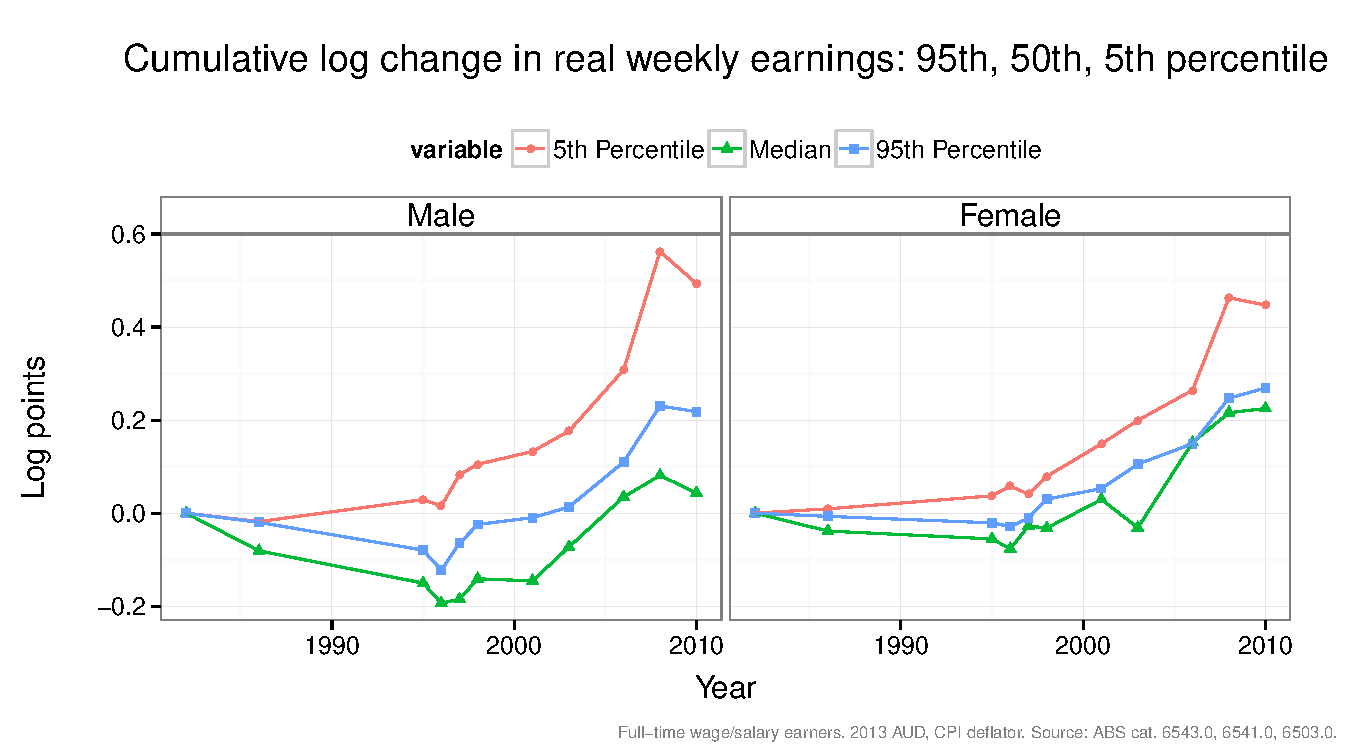
\includegraphics[width=\textwidth]{../figure/wage_change_time.pdf}
  \caption{Cumulative log change in real weekly earnings, 5th, 50th and 95th percentiles, 1982-2010. Full-time workers whose main sources of income are wages and salaries are shown. Notice that real wage growth has been non-monotone for males in lower percentiles. Source: Survey of Income and Housing.}
  \label{fig:changetime}
\end{figure}

This uneven pattern of job growth suggests that some property of middle-skill jobs, not present in low- and high-skill jobs, is responsible for this observed stagnation. In order to understand these differences, a new analytical framework is required.

Technology as a substitute, as well as a complement. President Eliot of Harvard, ``No man should be employed at a task a machine can perform'' \cite{Nordhaus2007}

\section{An Alternative Approach: `Jobs' and `Tasks'}

The neoclassical production function, which views aggregate economic output as a simple function of inputs such as capital and labor, does not consider the specifics of the processes which produced that output \citep{Acemoglu2011}. Although the canonical approach has been very successful in explaining aggregate output levels, it is not sensitive to qualitative changes in the nature of production such as changes in the technology which produce output. 

% note: production function appropriate for manufacturing; not service economy

% q-complements, versus substitutes

% insight: "what computers do"

The {\em task approach}, a research program initiated by \citet{Levy2003}, presents an alternative perspective to the standard neoclassical production function. Rather than viewing output as a direct function of resource inputs, it separates the tasks performed by labor and technology, allowing  substitutions between factors \citep{Autor2013,Acemoglu2011}. 

The task approach facilitates the inclusion of worker \emph{skills} in model. For the purposes of this analysis, we follow \citet{Autor2013} in viewing a \emph{task} as a discrete unit of work, which may be used to create final goods and services, and a worker's \emph{skill}, as the stock of capabilities for the execution of those tasks. Importantly, under this framework, the allocation of workers' skills to tasks is considered endogenous to the model: heterogeneous workers apply their skills to tasks where they enjoy a competitive advantage.

Under this framework, the performance of tasks is not confined to human workers. Since the industrial revolution, investments in labor-saving capital by firms has seen a dramatic change in the performance of repetitive tasks. The pace of technical change has been continual: as automated looms replaced hand-weavers in the 18th century, so too are cheap computers replacing administrative clerks and service workers in the 21st century.

The level and price of task-performing labor can be 
viewed as an outcome of the demand for particular tasks from workers and machine capital, and the supply of task-performing labor and capital. Unlike the canonical model, where technology is viewed as factor-augmenting,  technology can therefore be viewed as substitutes for some tasks, and complements for others. Thus firms are able to substitute between capital and human workers for the execution of tasks.

\section{ICT and Routinization}

In recent decades, the most important source of labor-saving capital has been information and computer technology (ICT). As the real cost of computation has fallen precipitously over the 20th century, computers have been able to execute a wider range of tasks at a lower cost. In the presence of falling costs of ICT, the question of work force polarization can thus be framed as an outcome of a decline in the real cost of computing capital, relative to the wage cost of human workers performing similar tasks.

Computers, despite their sophistication, are only capable of performing a very limited set of simple, routine tasks. They excel at processes which require calculation and simple symbolic manipulation, and are not prone to the same types of errors as human workers. It is this fact which has led to their widespread adoption in automated tellers and a wide range of electronic service delivery which were formerly the domain of human personnel. Yet, any task that requires abstract thought or physical coordination, however elementary they may appear to a human worker, is out of reach for a computer. Activities such as stacking shelves or driving a taxi are areas in which, for the moment at least, human workers enjoy a competitive advantage \citet{Levy2003}. 

Non-routine tasks, on the other hand, may improve, rather than replace, the efficiency of human workers. Indeed, as \citet{Borland2004} found by studying the computer knowledge of a cross-section of Australian workers surveyed in 1992, computer knowledge accrues a skill premium of around 10\%.

Thus computing capital is a complement to some kinds of task-performing labor, and a substitute for others. As \citet{Levy2003} show, in the United States between 1960 and 1998, computerization led to a substitution in the observed levels of employment, away from routine tasks and toward cognitive tasks. Likewise, \citet{Goos2007} show a similar trend in the United Kingdom: between 1975 and 2003, they find a increase in the number of ``lovely'' (high-skill, high-wage) jobs and ``lousy'' (low-wage, low-skill) jobs, but a relative decrease in the number of ``middling'' jobs. In a subsequent paper, a similar pattern was found for Continental Europe \citep{Goos2009}.

%It is therefore plausible, that the widespread adoption of ICT is a major driving force behind compositional changes in the workforce. 



Major shortcoming in study: complements to computer technology ignored. Except for specialised applications, hardware produced in 2013 unlikely to perform tasks that were impossible on machines available in 1981. Rather, complement of software, algorithms (which are usually non-rival goods), are not captured by industry capital investment on quality-adjusted terms.



\printbibliography

\end{document}

%%% Local Variables: 
%%% mode: latex
%%% End: 
